%\documentclass[a4paper]{article}
\usepackage[utf8]{inputenc}
\usepackage[spanish, es-tabla, es-noshorthands]{babel}
\usepackage[table,xcdraw]{xcolor}
\usepackage[a4paper, footnotesep=1.25cm, headheight=1.25cm, top=2.54cm, left=2.54cm, bottom=2.54cm, right=2.54cm]{geometry}
%\geometry{showframe}

%\usepackage{wrapfig}			%Wrap figure in text
\usepackage[export]{adjustbox}	%Move images
\usepackage{changepage}			%Move tables

\usepackage{tikz}
\usepackage{amsmath}
\usepackage{amsfonts}
\usepackage{amssymb}
\usepackage{float}
\usepackage{graphicx}
\usepackage{caption}
\usepackage{subcaption}
\usepackage{multicol}
\usepackage{multirow}
\usepackage{wrapfig}
\setlength{\doublerulesep}{\arrayrulewidth}
\usepackage{booktabs}
\usepackage[numbib, nottoc, notlot, notlof]{tocbibind}

\usepackage{hyperref}
\hypersetup{
    colorlinks=true,
    linkcolor=blue,
    filecolor=magenta,      
    urlcolor=blue,
    citecolor=blue,    
}

%Change Font Size

% #1 = size, #2 = text
\newcommand{\setparagraphsize}[2]{{\fontsize{#1}{6}\selectfont#2 \par}}		%Cambia el size de todo el parrafo
\newcommand{\setlinesize}[2]{{\fontsize{#1}{6}\selectfont#2}}				%Cambia el font de una oración

\newcommand{\note}[1]{
	\begin{center}
		\huge{ \textcolor{red}{#1} }
	\end{center}
}

%FONTS (IMPORTANTE): Compilar en XeLaTex o LuaLaTeX
\usepackage{anyfontsize}	%Font size
\usepackage{fontspec}		%Font type

\usepackage{etoolbox}
\usepackage{todonotes}

\newcommand{\observacion}[2]{  \ifnumequal{1}{#1}{ { \todo[inline,backgroundcolor=red!25,bordercolor=red!100]{\textbf{Observación: #2}} } }{  }  }

\setcounter{topnumber}{2}
\setcounter{bottomnumber}{2}
\setcounter{totalnumber}{4}
\renewcommand{\topfraction}{0.85}
\renewcommand{\bottomfraction}{0.85}
\renewcommand{\textfraction}{0.15}
\renewcommand{\floatpagefraction}{0.8}
\renewcommand{\textfraction}{0.1}
\setlength{\floatsep}{5pt plus 2pt minus 2pt}
\setlength{\textfloatsep}{5pt plus 2pt minus 2pt}
\setlength{\intextsep}{5pt plus 2pt minus 2pt}

\newcommand{\quotes}[1]{``#1''}
\usepackage{array}
\newcolumntype{C}[1]{>{\centering\let\newline\\\arraybackslash\hspace{0pt}}m{#1}}
\usepackage[american]{circuitikz}
\usetikzlibrary{calc}
\usepackage{fancyhdr}
\usepackage{units} 

\graphicspath{{../Control de posición no lineal/}{../Control de fuerza no lineal/}{../Control híbrido no lineal/}{../Referencias/}{../Deducción de modelo/}{../Conclusiones/}}

\pagestyle{fancy}
\fancyhf{}
\lhead{22.99 - Automación Industrial}
\rhead{Lambertucci, Londero B., Maselli, Mechoulam}
\rfoot{Página \thepage}

%Items con bullets y no cuadrados
\renewcommand{\labelitemi}{\textbullet }

%%
%\begin{document}


\Subsection{Realimentaci\'on de Estados}

Partiendo del sistema con fricción de la simulación, se comprueba la controlabilidad de este de manera homóloga a la explicada en la Sección (\ref{sec:ctrbyobsv}). 




Luego, se realizó la realimentación de estados utilizando el comando \textit{place} de Matlab, colocando a los polos según la Tabla (\ref{tab:realim}).

\begin{table}[H]
\centering
\begin{tabular}{@{}cccccc@{}}
\toprule
\multicolumn{6}{c}{Posición de los Polos} \\ \midrule
-3   & -2.5   & -2.4  & -2  & -1.9  & -1.8  \\ \bottomrule
\end{tabular}
\end{table}
\label{tab:realim}

La posición de los polos fue seleccionada de manera tal que el control sea rápido, pero no lo suficientemente rápido como para que la entrada no desvíe demasiado al sistema del punto de trabajo, lo cual haría que este se desestabilice ya que se está utilizando una técnica de control lineal en un sistema intrínsecamente no lineal.
Quedando entonces las ganancias de realimentación de la siguiente manera

\begin{table}[H]
\centering
\begin{tabular}{@{}cccccc@{}}
\toprule
\multicolumn{6}{c}{Ganancias}                    \\ \midrule
2.63 & 20.81 & 517.25 & 7.36 & 74.88 & 94.07 \\ \bottomrule
\end{tabular}
\end{table}
Se puede observar que el valor de las ganancias para el realimentador son relativamente bajas, por lo que su implementación en un dsp es mas sencillo.
Se puede observar en la Figura (\ref{fig:realim}) la simulación en bloques implementada en Simulink.

\begin{figure}[H]
	\centering
	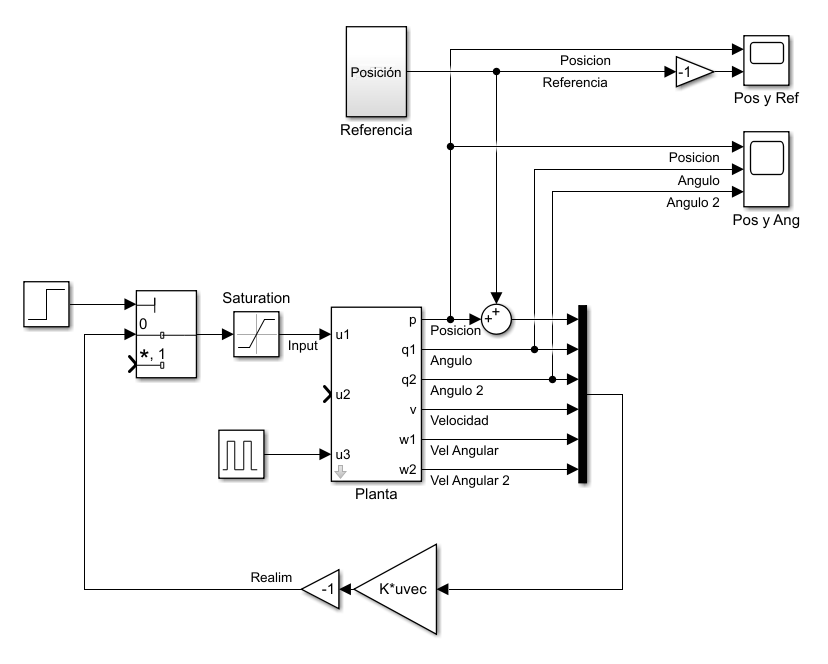
\includegraphics[width=\linewidth]{../Modelo de Control/ImagenesModelo de Control/realim.png}
	\caption{Simulación en bloques de la realimentación de estados.}	
	\label{fig:realim}
\end{figure}

\Subsection{Observador}

Como paso siguiente, se implementó una realimentación de estados con observador. Para esto, se comprobó la observabilidad del sistema con fricción, midiendo la posición del carrito y ambas posiciones angulares para estimar las variables del sistema restantes.

Se decidió colocar los polos del observador de manera tal que estos sean mucho más rápidos que los del sistema. Esto es para que la señal error entre las variables de estado y las estimaciones del observador converga rápidamente a cero. De esta manera, quedaron los polos del observador colocados según la Tabla (\ref{tab:obsv}).

\begin{table}[H]
\centering
\begin{tabular}{@{}cccccc@{}}
\toprule
\multicolumn{6}{c}{Posición de los Polos del Observador} \\ \midrule
-30    & -25    & -24    & -20    & -19    & -18   \\ \bottomrule
\end{tabular}
\end{table}
\label{tab:obsv}

por lo que las ganancias del observador quedan

\begin{table}[H]
\centering
\begin{tabular}{@{}cccccc@{}}
\toprule
\multicolumn{6}{c}{Ganancias}                    \\ \midrule
47.18 & 3.05  & 0.88  & 528.29 & 60.25  & 18.75  \\
2.16  & 43.35 & 0.73  & 40     & 468.40 & 12.29  \\
0.40  & 0.80  & 43.02 & 6.67   & 22.13  & 450.94 \\ \bottomrule
\end{tabular}
\end{table}
Cabe destacar que el valor de las ganancias para el observador son relativamente bajas, por lo que su implementación en un dsp es mas sencillo.

Se puede observar en la Figura (\ref{fig:obsv}) la simulación en bloques implementada en Simulink.

\begin{figure}[H]
	\centering
	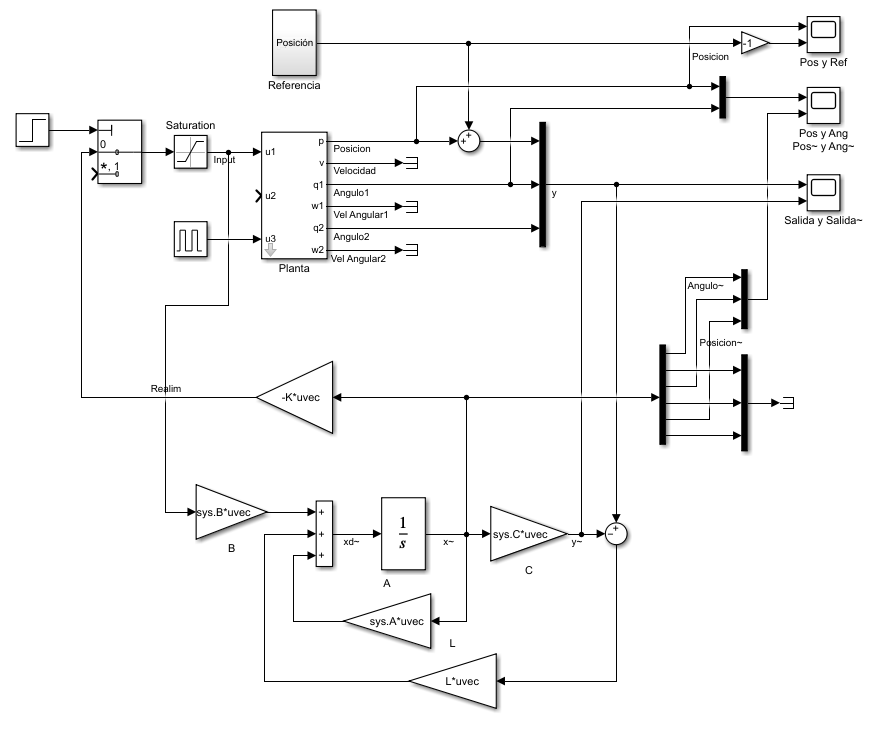
\includegraphics[width=\linewidth]{../Modelo de Control/ImagenesModelo de Control/obsv.png}
	\caption{Simulación en bloques de la realimentación de estados con observador.}	
	\label{fig:obsv}
\end{figure}

\Subsection{Discretizaci\'on}

Como último paso, se decidió pasar a tiempo discreto el sistema original con fricción utilizando la aproximación de Tustin con una tasa de muestreo de $30 \ ms$. Así quedando

\begin{equation}
 A = \begin{bmatrix}
1 &  -0.0010  & 0.0001 & 0.0250 &  0      & 0\\
0 &  1.0051  & -0.0040 & 0     &  0.0249 & 0.0002\\
0 &  -0.0062 & 1.0109  & 0     &  0.0002 & 0.0245\\
0 &  -0.0790  & 0.0092 & 1     &  0.0004 & -0.0015\\
0 &  0.4114  & -0.3190 & 0     &  0.9938 & 0.0173\\
0 &  -0.4971 & 0.8714 & 0     &  0.0151 & 0.9624
\end{bmatrix}
\end{equation}
\begin{equation}
 B = \begin{bmatrix}
0.0001 \\
-0.0001 \\
0.0001 \\
0.0047 \\
-0.0060 \\
0.0072
\end{bmatrix}
\end{equation}
\begin{equation}
 C = \begin{bmatrix}
1 &  -0.0005  & 0.0001 & 0.0125 &  0      & 0\\
0 &  1.0026  & -0.0020 & 0     &  0.0125 & 0.0001\\
0 &  -0.0031 & 1.0054  & 0     &  0.0001 & 0.0123
\end{bmatrix}
\end{equation}
\begin{equation}
 D = \begin{bmatrix}
0.2952 \cdot 10^{-4} \\
-0.3748 \cdot 10^{-4} \\
0.4529  \cdot 10^{-4}
\end{bmatrix}
\end{equation}

para luego realizar la realimentación de estados con observador, midiendo la posición del carrito y las posiciones angulares. Los polos se colocaron de manera siguiente

\begin{table}[H]
\centering
\begin{tabular}{@{}cccccc@{}}
\toprule
\multicolumn{6}{c}{Posición de los Polos (Plano Z)}                \\ \midrule
0.9560    & 0.9531    & 0.9503    & 0.9418   & 0.9389   & 0.9361   \\ \midrule
\multicolumn{6}{c}{Posición de los Polos del Observador (Plano Z)} \\ \midrule
0.4066    & 0.3829    & 0.3606    & 0.3012   & 0.2837   & 0.2671   \\ \bottomrule
\end{tabular}
\end{table}

quedando las ganancias de realimentación

\begin{table}[H]
\centering
\begin{tabular}{@{}clllll@{}}
\toprule
\multicolumn{6}{c}{Ganancias de Realimentación}                           \\ \midrule
0.7006 & \multicolumn{1}{c}{-34.1842} & \multicolumn{1}{c}{339.4479} & \multicolumn{1}{c}{2.3704}  & \multicolumn{1}{c}{34.6514} & \multicolumn{1}{c}{56.0334} \\ \midrule
\multicolumn{6}{c}{Ganancias de Realimentación del Observador}            \\ \midrule
1.4308 & \multicolumn{1}{c}{0.0081}   & \multicolumn{1}{c}{0.0018}   & \multicolumn{1}{c}{28.9658} & \multicolumn{1}{c}{0.4876}  & \multicolumn{1}{c}{0.1119}  \\
\multicolumn{1}{l}{0.0061} & 1.4318 & 0.0063 & 0.3489 & 29.0873 & 0.4613  \\
\multicolumn{1}{l}{0.0007} & 0.0071 & 1.4153 & 0.0161 & 0.6202  & 27.7099 \\ \bottomrule
\end{tabular}
\end{table}
Aquí las ganancias varían entre $10^2$ y $10^-4$ por lo que el realizar cuentas con estos en un dsp resulta sencillo.
Se puede observar en la Figura (\ref{fig:obsv_disc}) la simulación en bloques implementada en Simulink.

\begin{figure}[H]
	\centering
	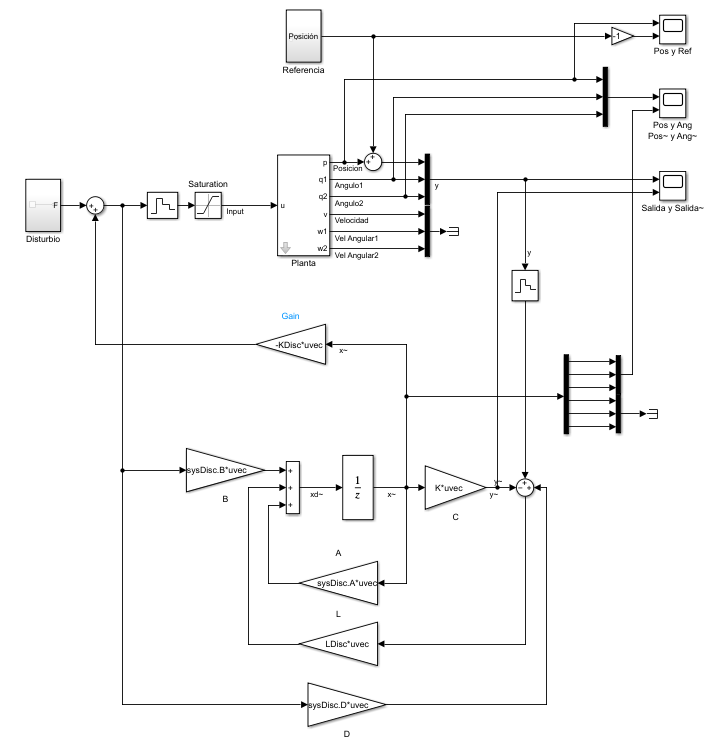
\includegraphics[width=\linewidth]{../Modelo de Control/ImagenesModelo de Control/obsv_disc.png}
	\caption{Simulación en bloques de la realimentación de estados con observador discreto.}	
	\label{fig:obsv_disc}
\end{figure}

\Subsection{Integral}

PENDIENTE

%\end{document}